\documentclass[a4paper,12pt]{article}

% don't forget the document class, generally : \documentclass[a4paper,12pt]{article}

\usepackage[utf8]{inputenc}
\usepackage[french]{babel}
\usepackage{graphicx}
\usepackage{gensymb}
\usepackage{amsmath}
\usepackage{float}
\usepackage{scrextend}
\usepackage{caption} 
\usepackage{siunitx}
\usepackage{enumitem}
\usepackage{amsthm}
\usepackage{fancyhdr}
\usepackage{amssymb}
\usepackage{wrapfig}
\usepackage{geometry}
\usepackage{standalone}
\usepackage{import}
\usepackage[usenames, dvipsnames]{color}

 \usepackage{biblatex} % manages bibliography and references
\addbibresource{sample.bib}


\geometry{hmargin=1in, vmargin=1in}

 \newenvironment{absolutelynopagebreak}
 {\par\nobreak\vfil\penalty0\vfilneg
 \vtop\bgroup}
 {\par\xdef\tpd{\the\prevdepth}\egroup
 \prevdepth=\tpd}
 
 \pagestyle{fancy}                        
\fancyhf{}                               
\fancyhf[HL]{Application des maths}                
\fancyhf[HR]{Géométrie euclidienne}             
\fancyhf[FC]{\thepage/\pageref{Lastpage}}
 
\newtheorem{definition}{Définition}[section]
\newtheorem{theorem}{Théorème}
\newtheorem{corollary}{Corollaire}[theorem]
\newtheorem{lemma}[theorem]{Lemme}
\newtheorem*{hyp}{Hypothèse}
\newtheorem*{concl}{Conclusion}
\newtheorem*{remark}{Remarque}

\captionsetup{format=default,labelformat=simple,labelsep=colon,
justification=justified,font={sf,small},labelfont=bf,
textfont=default} 



\begin{document}

\pagebreak
\subsection{Troisième cas d'isométrie des triangles}
\begin{theorem}
Deux triangles qui ont respectivement les trois côtés isométriques sont isométriques.
\end{theorem}
\begin{proof}
Nous considérons deux triangles $a_1b_1c_1$ et $a_2b_2c_2$.

\begin{figure}[H]
    \centering
    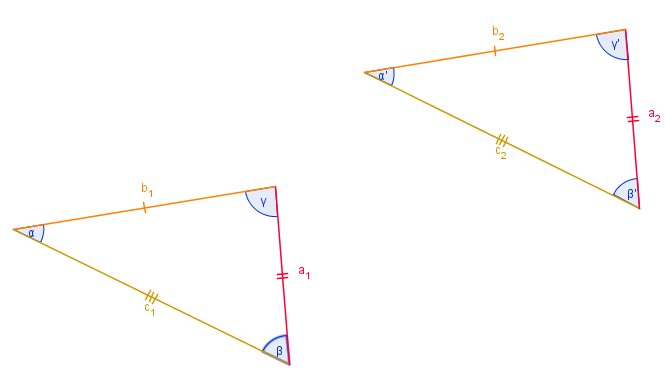
\includegraphics[scale=0.6]{theorems/isom3/Cas_3.PNG}
\end{figure}

 \begin{hyp}
     $a_1\equiv a_2$,
     $b_1\equiv b_2$ et
     $c_1\equiv c_2$
 \end{hyp}
 \begin{concl}
     $\alpha \equiv \alpha'$,
     $\beta \equiv \beta'$ et
     $\gamma \equiv \gamma'$
 \end{concl}
 Nous rassemblons les deux triangles en un quadrilatère en superposant $c_1$ et $c_2$. 
 
 \begin{figure}[H]
    \centering
    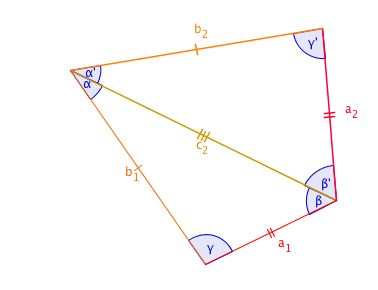
\includegraphics[scale=0.6]{theorems/isom3/Cas3_2.png}
\end{figure}
 
 Puis nous relions les sommets en $\gamma$ et $\gamma'$, nous nommons ce segment $h$. Ainsi, nous obtenons deux triangles qui sont isocèles $\triangle a_1a_2h$ et $\triangle b_1b_2h$ ($a_1\equiv a_2$ pour $\triangle a_1a_2h$ et $b_1\equiv b_2$ pour $\triangle b_1b_2h$, voir section 6.3) ce qui signifie que $\theta_1 \equiv \theta_2$ et que $\theta_3 \equiv \theta_4$.
 
 
 \begin{figure}[H]
    \centering
    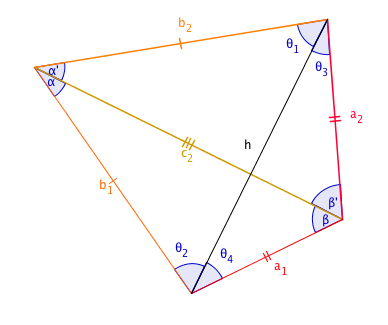
\includegraphics[scale=0.6]{theorems/isom3/Cas3_3.png}
\end{figure}

 
 
 Finalement, comme $\alpha \equiv \theta_1 + \theta_2$ et $\alpha' \equiv \theta_3 + \theta_4$, nous avons démontré que $\alpha \equiv \alpha'$. Les deux triangles $a_1b_1c_1$ et $a_2b_2c_2$ sont donc isométriques (axiome III).
\end{proof}

\end{document}
